\documentclass{beamer}
\usepackage[utf8]{inputenc}
\usetheme{Singapore}
\usecolortheme{default}
\beamertemplatenavigationsymbolsempty


\title[Genetic algorithm for QSVM] 
{Genetic algorithm for Quantum Support Vector Machines}



\author[Lorenzo Tasca]
{Lorenzo Tasca}
 

\date[25/11/2024] 
{25 Novembre 2024}

\logo{
\includegraphics[height=1cm]{images/logo.png}}

\begin{document}

\frame{\titlepage}

\begin{frame}
\frametitle{Quantum Machine Learning}
\centering
\begin{figure}
      
\includegraphics[width=1.1\textwidth]{images/1.png}
     \end{figure}
\end{frame}



\begin{frame}
  \frametitle{Support Vector Machine}
    \begin{itemize}
      \item     La Support Vector Machine è un algoritmo supervisionato di classificazione binaria. 
    \end{itemize}
      \begin{figure}
            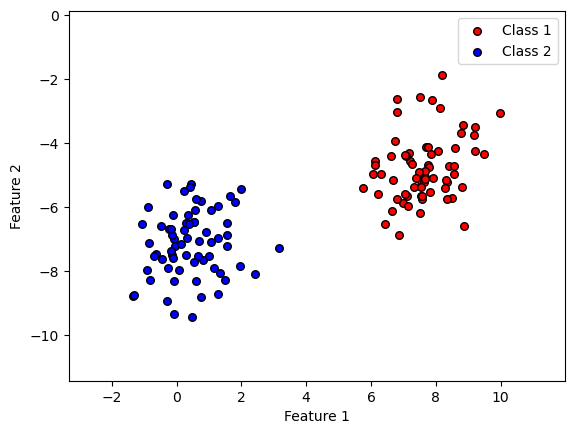
\includegraphics[width=0.7\textwidth]{images/classicaldata.png}
       \end{figure}
  \end{frame}



  \begin{frame}
    \frametitle{Support Vector Machine}
      \begin{itemize}
        \item L'algoritmo trova il massimo margine separatore tra le classi. 
      \end{itemize}
        \begin{figure}
              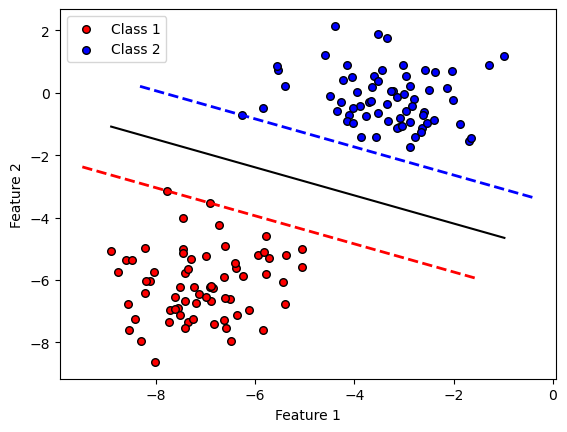
\includegraphics[width=0.7\textwidth]{images/classicalsvm.png}
         \end{figure}
    \end{frame}


    \begin{frame}
      \frametitle{Support Vector Machine}
        \begin{itemize}
          \item Per farlo utilizza solo i prodotti scalari tra i dati $\langle \mathbf{x}_i, \mathbf{x}_j\rangle$.  
        \end{itemize}
          \begin{figure}
                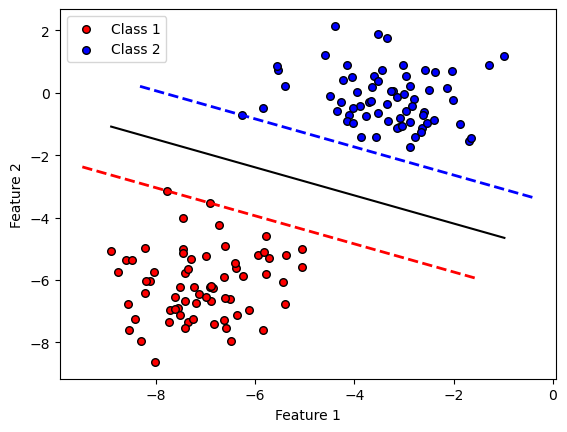
\includegraphics[width=0.7\textwidth]{images/classicalsvm.png}
           \end{figure}
      \end{frame}


\begin{frame}
  \frametitle{Kernel Support Vector Machine}
  
  \begin{itemize}
    \item Nel caso in cui i dati non siano linearmente separabili?
  \end{itemize}
     
        \begin{figure}
          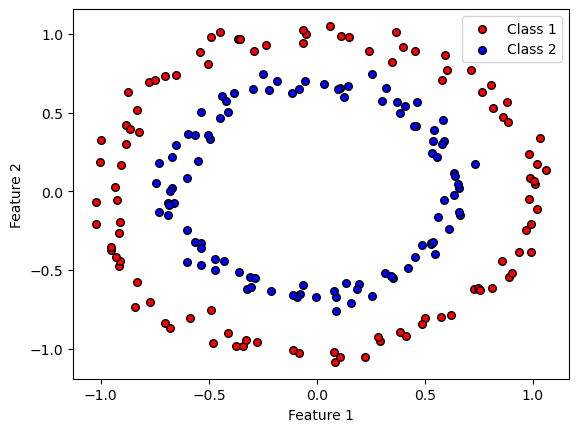
\includegraphics[width=0.7\textwidth]{images/circles.png}
        \end{figure}
        
\end{frame}

\begin{frame}
  \frametitle{Kernel Support Vector Machine}
  
  \begin{itemize}
    \item È possibile applicare una feature map $\phi(\mathbf{x})$.
  \end{itemize}
     
        \begin{figure}
          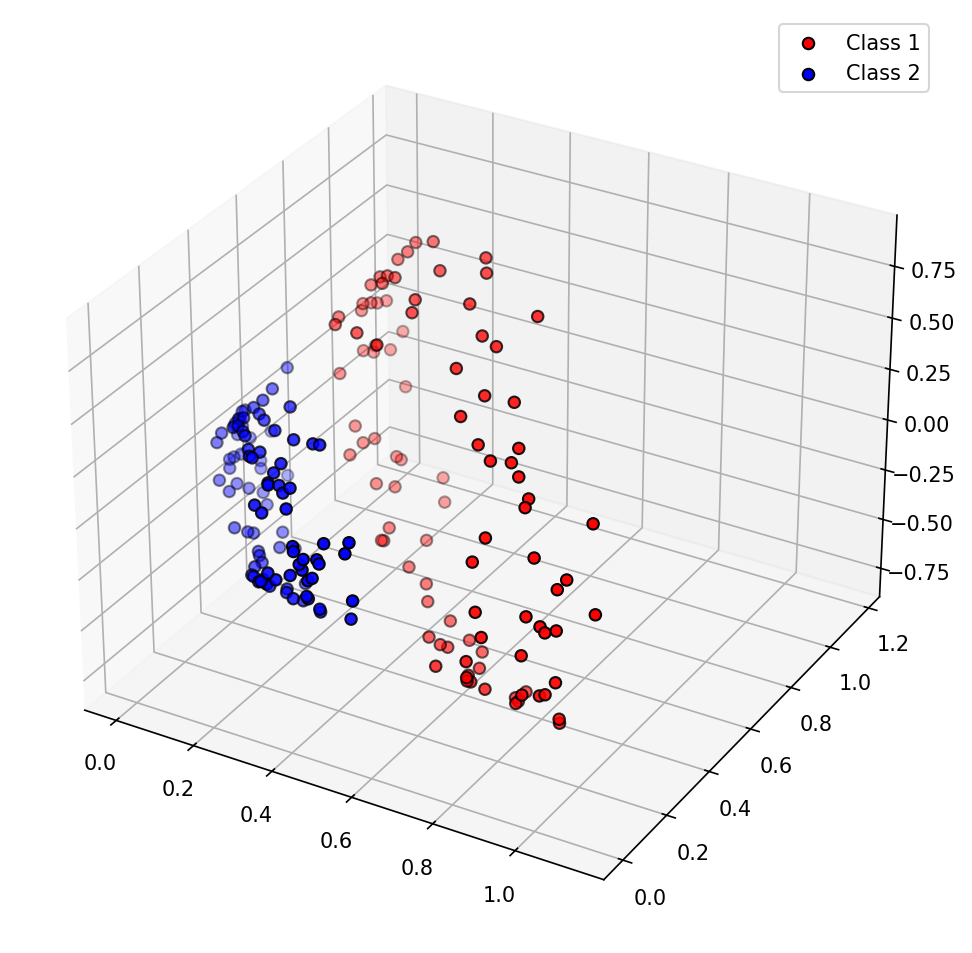
\includegraphics[width=0.6\textwidth]{images/circles3d.png}
        \end{figure}
        
\end{frame}

\begin{frame}
  \frametitle{Kernel Support Vector Machine}
  
  \begin{itemize}
    \item L'algoritmo è interessato solo a $K_{ij}=\langle \phi(\mathbf{x}_i), \phi(\mathbf{x}_j) \rangle$.

  \end{itemize}
     
        \begin{figure}
          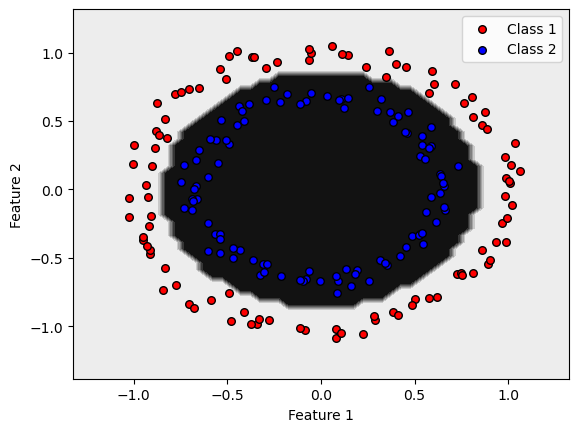
\includegraphics[width=0.7\textwidth]{images/separatedcircle.png}
        \end{figure}
        
\end{frame}








\begin{frame}

  \frametitle{Quantum Support Vector Machine}
  
  \begin{columns}
    \column{0.5\textwidth}
  
    \begin{itemize}
      \item<1-> La feature map diventa un circuito quantistico parametrizzato. \\\,
          \item<2-> $|\phi(\mathbf{x})\rangle=U(\mathbf{x})|0\rangle^{\otimes n}$.\\\,
          \item<3->  $K_{ij}=\langle \phi(\mathbf{x}_i)| \phi(\mathbf{x}_j) \rangle.$
          \end{itemize}
    
    \column{0.5\textwidth}
    \only{\begin{figure}
          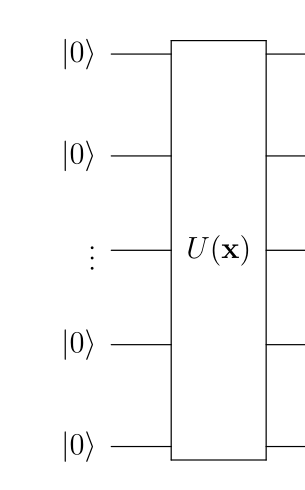
\includegraphics[width=0.7\textwidth]{images/Pasted image.png}
     \end{figure}}<1>
     \only{\begin{figure}
      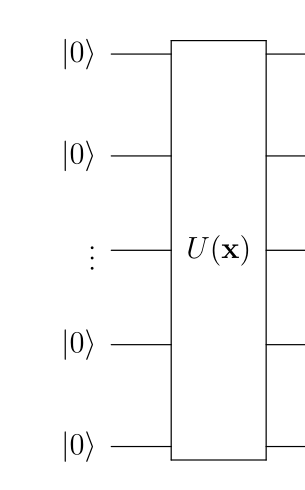
\includegraphics[width=0.7\textwidth]{images/Pasted image.png}
 \end{figure}}<2>
     \only{\begin{figure}
      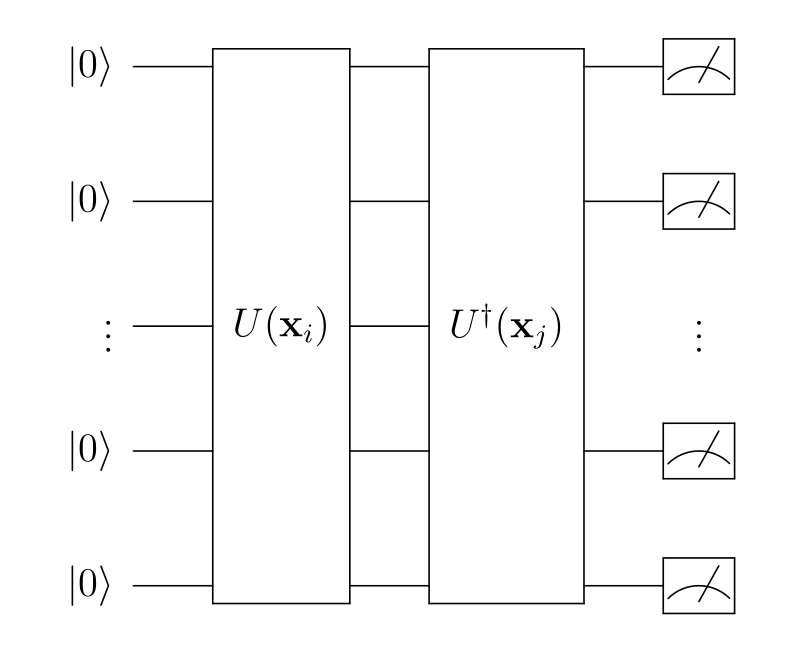
\includegraphics[width=\textwidth]{images/Pasted image (2).png}
 \end{figure}}<3>


    
    \end{columns}

\end{frame}


\begin{frame}
  \frametitle{Quantum Feature Maps}

  \begin{columns}
    \column{0.5\textwidth}
  
    \begin{itemize}
      \item<1-> Ci sono moltissime scelte possibili di circuiti. Un esempio è la ZZ feature map.
          \item<2-> La QSVM mostra il potenziale di separare complicati dataset, con pattern complessi.  
          \item[]<3->  
          \item<4-> Questi dataset non sono gestibili coi kernel classici. 
          
          \end{itemize}
    
    \column{0.5\textwidth}
    \only{\begin{figure}
          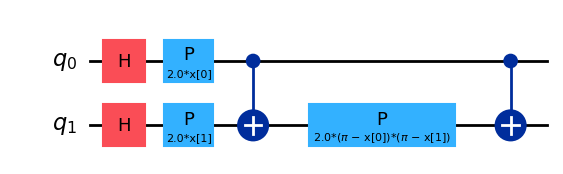
\includegraphics[width=1\textwidth]{images/ZZ.png}
     \end{figure}}<1>
     \only{\begin{figure}
      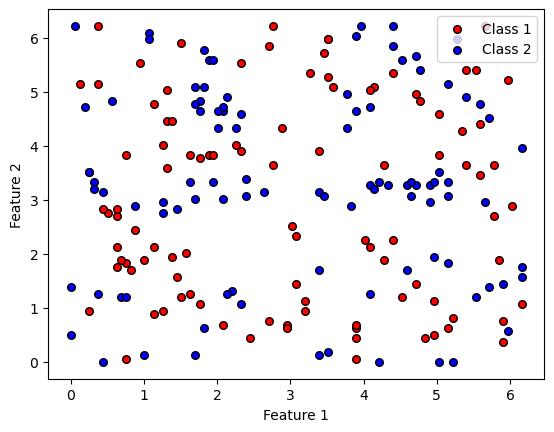
\includegraphics[width=\textwidth]{images/adhoc.png}
 \end{figure}}<2>
 \only{\begin{figure}
  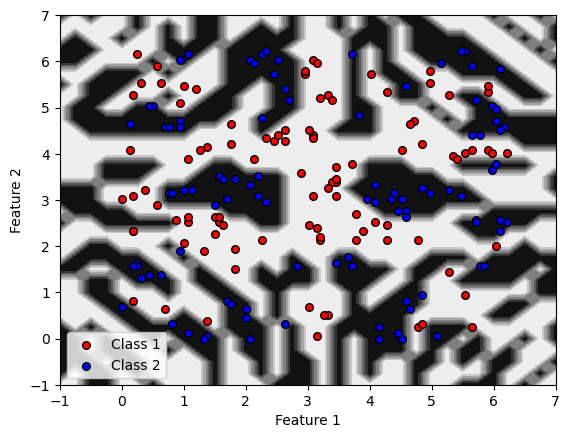
\includegraphics[width=\textwidth]{images/adhoczz.png}
\end{figure}}<3>
\only{\begin{figure}
  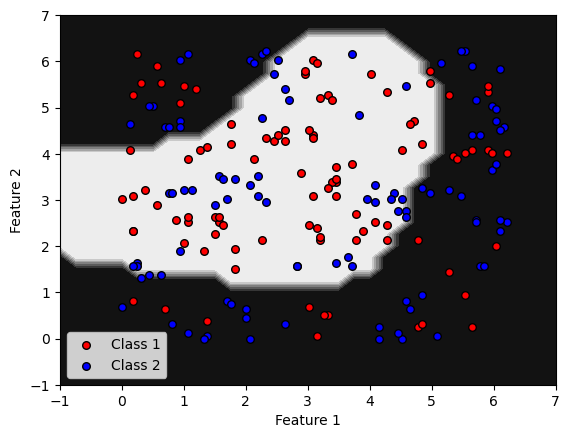
\includegraphics[width=\textwidth]{images/adhocrbf.png}
\end{figure}}<4>
    
    \end{columns}

\end{frame}



\begin{frame}
  \frametitle{Quantum Feature Maps}

  \begin{columns}
    \column{0.5\textwidth}
  
    \begin{itemize}
      \item<1-> Nonostante le grandi potenzialità, la scelta della feature map si rivela molto delicata.
          \item<2-> Una scelta non congeniale porta a performance pessime, con accuretezze anche inferiori al 50\%. 
      
          \item<3-> Il problema è che non ci sono regole generali valide per la scelta del circuito. 
          
          \end{itemize}
    
    \column{0.5\textwidth}

     \only{\begin{figure}
      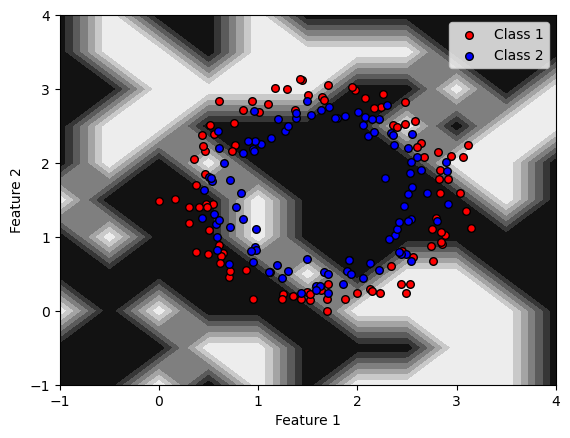
\includegraphics[width=\textwidth]{images/failcircle.png}
 \end{figure}}<2>
 \only{\begin{figure}
  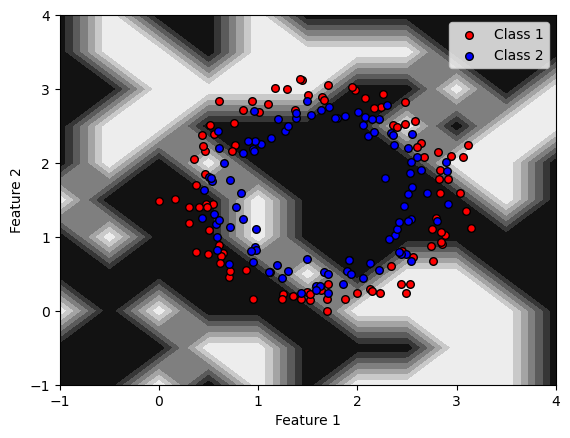
\includegraphics[width=\textwidth]{images/failcircle.png}
\end{figure}}<3>

    
    \end{columns}

\end{frame}



\end{document}